\documentclass[10pt]{article}

\usepackage[a4paper, left=2cm, right=2cm]{geometry} % A4 paper size and thin margins

\usepackage{xcolor} % Required for specifying custom colours
\definecolor{grey}{rgb}{0.9,0.9,0.9} % Colour of the box surrounding the title

\usepackage{graphicx}
\usepackage[colorlinks=true, allcolors=black]{hyperref}
\usepackage{indentfirst}
\setlength{\parindent}{2em}
\usepackage{multirow}
\usepackage[normalem]{ulem}

\usepackage[utf8]{inputenc} % Required for inputting international characters
\usepackage[T1]{fontenc} % Output font encoding for international characters
\usepackage[sfdefault]{ClearSans} % Use the Clear Sans font (sans serif)
%\usepackage{XCharter} % Use the XCharter font (serif)

\begin{document}
%----------------------------------------------------------------------------------------
%	TITLE PAGE
%----------------------------------------------------------------------------------------

\begin{titlepage} % Suppresses displaying the page number on the title page and the subsequent page counts as page 1
	
	%------------------------------------------------
	%	Grey title box
	%------------------------------------------------
	
	\colorbox{grey}{
		\parbox[t]{1.1\textwidth}{ % Outer full width box
			\parbox[t]{1.02\textwidth}{ % Inner box for inner right text margin
				\raggedleft % Right align the text
				\fontsize{34pt}{40pt}\selectfont % Title font size, the first argument is the font size and the second is the line spacing, adjust depending on title length
				\vspace{0.7cm} % Space between the start of the title and the top of the grey box
				
				< Journey Assistant >\\
                Project Development Plan\\
                Version 1.0\\
				
				\vspace{0.7cm} % Space between the end of the title and the bottom of the grey box
			}
		}
	}
	
	\vfill % Space between the title box and author information
	
	%------------------------------------------------
	%	Author name and information
	%------------------------------------------------
	
	\parbox[t]{1\textwidth}{ % Box to inset this section slightly
		\raggedleft % Right align the text
		\large % Increase the font size
		{\Large Group Member}\\[4pt] % Extra space after name
        Yiwen Song\\
        Zhihui Xie\\
        Weizhe Wang\\
        Huangfei Jiang\\
        Haoping Chen\\
		% Institution Name\\[4pt] % Extra space before URL
		% \texttt{LaTeXTemplates.com}\\
		
		\hfill\rule{0.2\linewidth}{1pt}% Horizontal line, first argument width, second thickness
    }
    
	
\end{titlepage}

\newpage

\begin{center}
    {\LARGE Modification History}
    
    \begin{tabular}{|c|c|c|c|} 
        \hline 
        Date&Version&Description&Author\\
        \hline  
        2019-04-02&1.0&The first version of this document.&Yiwen Song\\
		\hline 
		 & & & \\
		\hline
		& & & \\
		\hline
		& & & \\
		\hline
    \end{tabular}    
\end{center}

\newpage

\tableofcontents
\newpage

\section{Intruduction}
\subsection{Purpose}
The purpose of this project development plan is to help the project developers clarify their jobs, deadlines and technical outlooks of this project. We expect all the project developers (or anyone who are involved in the development of this project) to know the development plan of our project.

\subsection{Background}
There are some statement we need to make before entering the main part.

\begin{itemize}
	\item[1.] The NAME of our software system is Journey Assistant.
	\item[2.] The project is our final project of Software Engineering course, developed by Yiwen Song, Zhihui Xie, Haoping Chen, Weizhe Wang and Huangfei Jiang of SEIEE, Shanghai Jiaotong University. The target user of our system is the travellers who are making their journey plans. 
	\item[3.] Our software system is an upgrade of the trip-recommendation system of Xiecheng, Tuyou, etc. We use automation algorithms to give journey plan recommendations, distinguished from the companies' manual recommendations.
\end{itemize}

\subsection{Definition}
Here we list some terms or abbreviations we will use in this file.

\begin{center}
\begin{tabular}{|c|c|c|} 
	\hline 
	Abbreviation&Term&Implication\\
	\hline  
	JAS&Journey Assistant System&Our Proposed System\\
	\hline 
	 &Android&An OS Developed by Google\\
	\hline
	OS&Operating System& \\
	\hline
	TCP/IP& &A Network Protocol\\
	\hline
\end{tabular}    
\end{center}

\subsection{Bibliography}
\begin{itemize}
	\item[1.] <Feasibility Study Report> (GB8567-88)
	\item[2.] <Object Oriented Software Engineering (Version 3)> (Tsinghua University Press)
	\item[3.] <Clean Code> (Posts \& Telecom Press)
	\item[4.] <Machine Learning> (Tsinghua University Press)
	\item[5.] <Object Oriented Software Engineering Practice Guidelines> 
\end{itemize}

\section{Project Outlook}
\subsection{Project Target and Job Contents}
The purpose of our project is to develop a software system that can automatically recommend journey plans and help the users customize a plan. The main jobs involved in this projects are:

\begin{itemize}
	\item[1.] Design a friendly user interface.
	\item[2.] Design a good recommendation algorithm.
	\item[3.] Implement the algorithm in a fast way in our software.
	\item[4.] Design an port for the users to give advice.
\end{itemize}

\subsection{Team Organization Pattern}
The organization pattern of our project team are listed as follows.

\begin{itemize}
	\item[1.] Yiwen Song is the team leader. Organizes all the jobs, and will participate in algorithm designing and implementation and UI designing.
	\item[2.] Zhihui Xie is in charge of technical works, including algorithm designing and implementation, API ports, etc.
	\item[3.] Haoping Chen will be in charge of the desgning works including art, texts and interface design.
	\item[4.] Huangfei Jiang will be in charge of the database construction works, who will be responsible for acquiring data from other companies' APIs, and maintaining our database.
	\item[5.] Weizhe Wang will be in charge of the optimization works, who gives advice to all aspects of jobs and help make our software become more efficient and user-friendly.  
\end{itemize}

\subsection{Pruduct}
\subsubsection{Programs}
The programs that will be delivered to the users are listed as follows.

\paragraph{\underline{The User-interface Module}} Coded with Java (complied to binary). Pakced in the main software program. This module is the manager of the user-interface, including login interface, destination-choosing interface, requirement-choosing interface and other display interfaces.

\paragraph{\underline{The Display-data Module}} Coded with C++ and Java (complied to binary). Packed in the main software program. The maps and figures needed are packed in folders and saved in the user's flash drive. This module receives the data from our server and display it to the user.

\paragraph{\underline{The Save-data Module}} Coded with Java (complied to binary). Packed in the main software program. This module saves key data to the user's device to enable offline-request.

\subsubsection{Files}
The files that will be delivered to the users are listed as follows.

\paragraph{\underline{The Operation Manual}} It tells the operations of our software.

\paragraph{\underline{The Service Agreement}} It orders the user to agree the protocols in order to use our software. 

\paragraph{\underline{Essential Figures and Videos}} Some essential figures and videos are kept in the user's device. Therefore, the user does not need to query the essential data every time they use the software. 


\subsubsection{Services}
The services that will be delivered to the users are listed as follows.

\paragraph{\underline{Application Maintainence}} Starts from installation, ends by uninstallation. 

\begin{itemize}
	\item Priority Level: Medium. 
	\item Service Due Date: None.
\end{itemize}

\paragraph{\underline{User Guide}} Given at the first time the user uses the application.

\begin{itemize}
	\item Priority Level: Low.
	\item Service Due Date: After the first use.
\end{itemize}

\paragraph{\underline{Bug Reporting}} Starts from installation.

\begin{itemize}
	\item Priority Level: High.
	\item Service Due Date: None.
\end{itemize}

\paragraph{\underline{Advice Port}} Starts from the first use.

\begin{itemize}
	\item Priority Level: Low.
	\item Service Due Date: None.
\end{itemize}

\subsubsection{Non-delivered Products}
The products that will NOT be delivered to the users are listed as follows.

\begin{itemize}
	\item[1.] The user database. Using MySQL. Saving the username, user info, and password.
	\item[2.] The recommendation and customization algorithm. Coded by Java. 
	\item[3.] Unessential figures and data.
\end{itemize}

\subsection{Acceptance Certificate Standard}
The whole system works well and stably, according to <Software Testing Standard> (GB15532-2008).

\subsection{Predicted Completion Time and Latest Delay}	
The project is predicted to be completed on 2019.6.23, and the delay will be no more than 1 week.

\section{Performance Plan}
\subsection{Split of Jobs and Division of Labor}

\begin{center}
	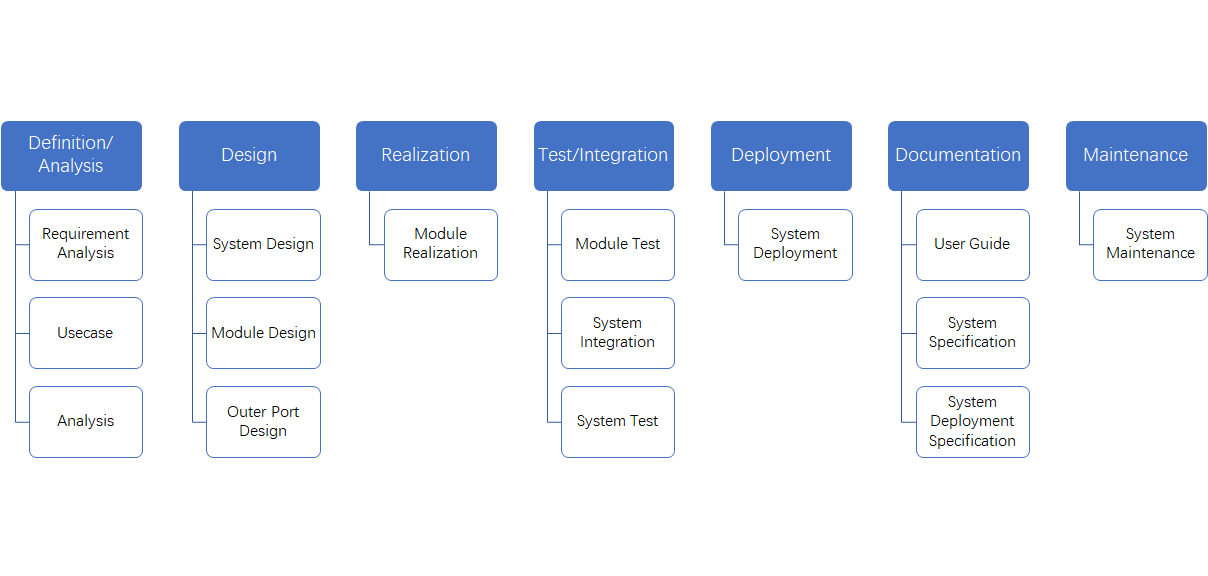
\includegraphics[width=12cm]{PP.png}

	\begin{tabular}{|c|c|c|} 
		\hline 
		\textbf{Project}&\textbf{Leader}&\textbf{Participating Members}\\
		\hline  
		Requirement Analysis&Weizhe Wang&Huangfei Jiang\\
		\hline 
		Use Case&Huangfei Jiang&Yiwen Song, Weizhe Wang\\
		\hline
		Analysis&Haoping Chen&Zhihui Xie\\
		\hline
		System Design&Yiwen Song&All\\
		\hline
		Module Design&Zhihui Xie&All\\
		\hline
		Outer Port Design&Zhihui Xie&Weizhe Wang, Huangfei Jiang\\
		\hline
		Module Realization&Yiwen Song&All others\\
		\hline
		Module Test&Weizhe Wang&Zhihui Xie, Haoping Chen\\
		\hline
		System Integration&Haoping Chen&All others\\
		\hline
		System Test&Huangfei Jiang&Weizhe Wang, Zhihui Xie\\
		\hline
		System Development&Yiwen Song&All others\\
		\hline
		User Guide&Haoping Chen&Weizhe Wang, Huangfei Jiang\\
		\hline
		System Specification&Yiwen Song&Haoping Chen, Weizhe Wang\\
		\hline
		System Development Specification&Yiwen Song&Weizhe Wang\\
		\hline
		System Maintainence&Weizhe Wang&All others\\
		\hline
	\end{tabular}    
\end{center}

\subsection{Phase Plans}
\begin{center}
	\begin{tabular}{|c|c|} 
		\hline 
		\textbf{Milestone Event}&\textbf{Predicted Time}\\
		\hline  
		Requirement Definition&2019.4.7\\
		\hline
		Software Architecture&2019.4.28\\
		\hline
		Module Development&2019.5.19\\
		\hline
		System Integration&2019.6.1\\
		\hline
		System Display&2019.6.9\\
		\hline
		System Deployment&2019.6.21\\
		\hline
		Project Completion&2019.6.23\\
		\hline
	\end{tabular}    

	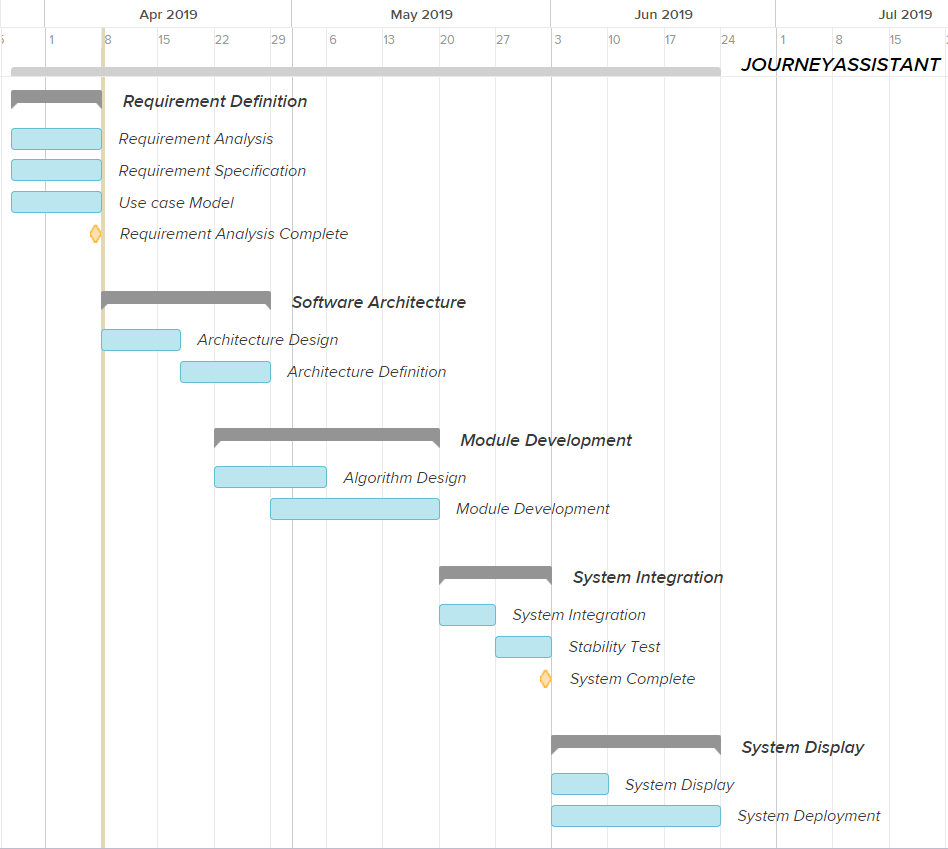
\includegraphics[width=12cm]{2.png}
\end{center}

\subsection{Budget}
We have a limited budget to complete the project, as our labor needs no salary. The main cost lies on the oursourcing work such as art design and server rent.

\subsection{Key Problem}
\begin{itemize}
	\item[1.] The safety of users' information. If the users' information were lost or stolen, it will cause greate economical loss and privacy cost.
	\item[2.] The capability and stability of databse. If the stability or capability of database is not enough, the system may fail at unpredictable time.
	\item[3.] Friendliness of user interface. A friendly user interface will attract more users.
	\item[4.] Easiness of using. A easy-using software will keep more users.
	\item[5.] The plan, communications, and technical restricts during our development. Our development progress may be delayed, prolonged or we may not be able to complete planned tasks.
\end{itemize}

\section{Technological Process Plan}
\subsection{Methodology, Tools and Techniques}
\begin{itemize}
	\item[1.] Our project is maily developed by Java, C++ and Python, use IDE Eclipse/IntelliJ, CLion, and PyCharm.
	\item[2.] The database is maily developed by the open-source database MySQL.
	\item[3.] We use structural development to split our whole system into several modules and develop them individually.
	\item[4.] We use fountain model for the life cycle of our project.
\end{itemize}

\subsection{Technical Standards}
The technical standards we will use in our development include:

\begin{itemize}
	\item[1.] Business Modeling Guide: <Business Modeling Guide> 
	\item[2.] UI Guide: Google Material Design
	\item[3.] Use case Modeling Guide: <Use-case Modeling Guide>
	\item[4.] Design Guide: Google Material Design
	\item[5.] Programming Guide: <Object Oriented Software Engineering>
	\item[6.] Testing Guide: <Software Testing Standard>, Pearson (GB15532-2008)
	\item[7.] Coding Scheme Guide: <Clean Code>, Robert C. Martin
\end{itemize}

\section{External Support Conditions}
\subsection{Jobs Performed by Users}
We need to users to create their account (sign up) the first time they use our software. Then their account will be saved in our database and they aren't required to do any further jobs. Other non-required jobs include bug reporting and giving advice.

\subsection{Jobs Performed by Other Companies}
We may use some API developed by other companies in our project. They include:

\begin{itemize}
	\item[1.] Map API supported by Gaode or Baidu Inc. 
	\item[2.] Scenary information API supported by MeituanDianping Inc.
	\item[3.] Tensorflow, a deep learning development kit, developed by Google Inc.
	\item[4.] Anaconda, a multi-functional kit for Python, developed by Anaconda Inc.
	\item[5.] Open-source web frameworks such as bootstrap.
	\item[6.] Other open-source codes developed by personal developers or small teams.
\end{itemize}

\section{Plan Keywords}
\begin{itemize}
	\item[1.] In the requirement management plan we will mainly focus on the requirement analysis, and make plans according to our ability to satisfy as much need as possible.

	\item[2.]In the progress control plan, the key point is to control the progress as planned during our development of our project
	The quality control plan is mainly about to improve our project quality in planned time.
	
	\item[3.]The risk management plan is mainly about reducing the risk during and after our completion of our project, and make plans before the accidents happen.
	
	\item[4.]	The equipment management plan is mainly about reducing the cost of our equipments under the constraints of quality control
	
	\item[5.]
	The system testing plan is mainly about finding as much bugs and repair them as possible before our software finally goes into the application market.
	
	\item[6.]
	The system acceptance plan is mainly about making a proper standard for our project. The standard should not be too hard to pass, but also not be too easy so that the software may not be friendly at last.
	
	\item[7.]
	The developer training plan is mainly about training developers to complete the tasks they should do.
	
	\item[8.]
	The system installation plan is mainly about finding a proper way to make a good sequence to install the system
\end{itemize}


%----------------------------------------------------------------------------------------

\end{document}

